\documentclass[dvisvgm]{standalone}
\usepackage{tikz} 

\definecolor{Acolor}{HTML}{466d9a}
\definecolor{Bcolor}{HTML}{99ced3} 
\definecolor{medgrey}{HTML}{A7AAAD} 

\begin{document}
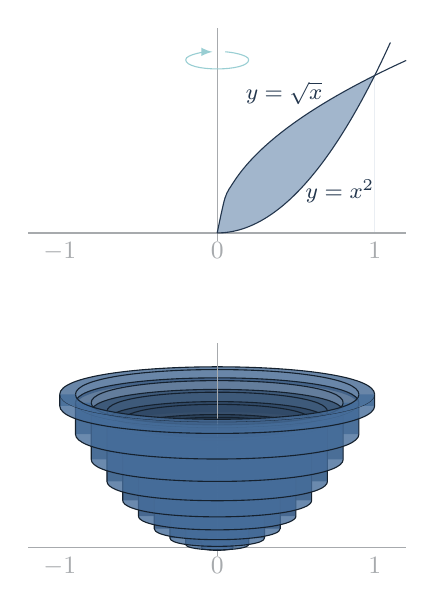
\begin{tikzpicture}[scale=2]
  \fill[domain=0:1,smooth,variable=\x,  Acolor,fill opacity=0.5]  plot ({\x},{sqrt(\x)})--(1,0)--(0,0);
  \fill[domain=0:1,smooth,variable=\x,  white,fill opacity=1]  plot ({\x},{\x*\x})--(1,0)--(0,0);

  \draw[medgrey](-1.2,0)--(1.2,0);
  \draw[medgrey](0,-0.05)--(0,1.3);

  \draw[Bcolor](-0.2,1.1) to[out=270, in=270,looseness=0.5] (0.2,1.1);
  \draw[Bcolor,-latex](-0.2,1.1) to[out=90, in=180,looseness=0.5] (-0.03,1.15);
  \draw[Bcolor](0.2,1.1) to[out=90, in=0,looseness=0.5] (0.05,1.15);

  \draw[domain=0:1.2,smooth,variable=\x,  ,Acolor!50!black]  plot ({\x},{sqrt(\x)});
  \draw[domain=0:1.1,smooth,variable=\x,  ,Acolor!50!black]  plot ({\x},{\x*\x});

  \node[below right,Acolor!50!black] at (0.5,0.4) {\footnotesize $y=x^2$};
  \node[above left,Acolor!50!black] at (0.73,0.75) {\footnotesize $y=\sqrt{x}$};

  \node[medgrey, below] at (1,0) {\small $1$};
  \node[medgrey, below] at (0,0) {\small $0$};
  \node[medgrey, below] at (-1,0) {\small $-1$};

  \begin{scope}[yshift=-2cm]
    \draw[ medgrey](-1.2,0)--(1.2,0);

    \foreach \x in {0.95,0.85,0.75,...,-0.05} {
    \pgfmathparse{\x*100}
      \fill[Acolor!\pgfmathresult!black,opacity=0.8](\x+0.05,{sqrt(\x)}) to[out=90, in=90,looseness=0.3] (-\x-0.05,{sqrt(\x)})--(-\x-0.05,{\x*\x})--(-\x+0.05,{\x*\x})to[out=90, in=90,looseness=0.3](\x-0.05,{\x*\x})--(\x+0.05,{\x*\x});
      \draw[thin,Acolor!30!black](\x+0.05,{sqrt(\x)}) to[out=90, in=90,looseness=0.3] (-\x-0.05,{sqrt(\x)});
      \draw[thin,Acolor!30!black] (-\x+0.05,{sqrt(\x)}) to[out=90,in=90,looseness=0.3] (\x-0.05,{sqrt(\x)});
    }
    \draw[ medgrey](0,-0.05)--(0,1.3);

    \foreach \x in {0.05,0.15,0.25,0.35,0.45,0.55,0.65,0.75,0.85,0.95} {
      \fill[Acolor,opacity=0.8](\x-0.05,{sqrt(\x)})--(\x+0.05,{sqrt(\x)})--(\x+0.05,{\x*\x}) to[out=270, in=270,looseness=0.3] (-\x-0.05,{\x*\x})--(-\x-0.05,{sqrt(\x)})--(-\x+0.05,{sqrt(\x)})to[out=270, in=270,looseness=0.3](\x-0.05,{sqrt(\x)});

      \draw[thin,Acolor!30!black] (\x+0.05,{sqrt(\x)})--(\x+0.05,{\x*\x}) to[out=270, in=270,looseness=0.3] (-\x-0.05,{\x*\x})--(-\x-0.05,{sqrt(\x)});
      \draw[thin,Acolor!30!black] (\x-0.05,{sqrt(\x)}) to[out=270, in=270,looseness=0.3] (-\x+0.05,{sqrt(\x)});
      \draw[ultra thin,Acolor!30!black] (\x+0.05,{sqrt(\x)}) to[out=270, in=270,looseness=0.3] (-\x-0.05,{sqrt(\x)});
    }
    \node[medgrey, below] at (1,0) {\small $1$};
    \node[medgrey, below] at (0,0) {\small $0$};
    \node[medgrey, below] at (-1,0) {\small $-1$};
  \end{scope}
\end{tikzpicture}
\end{document}
